\paragraph{IUE04.1 Modificar información de Practicante} \hspace{1cm}\\ 
\label{pant:IUE04.1} 

\textbf{\textcolor[rgb]{0, 0, 0.545098}{Objetivo}}\\
Esta pantalla permite al Entrenador modificar los datos del Practicante registrado.\\

\textbf{\textcolor[rgb]{0, 0, 0.545098}{Diseño}}\\
En la figura \ref{fig:IUE04.1} se muestra la pantalla \nameref{fig:IUE04.1}, por medio de la cual el Entrenador visualiza un formulario, el cual contiene los campos de registro de información, con los datos previamente guardados.\\

En la parte inferior se encuentran los botones Guardar y Cancelar,  los cuales corresponden a registrar los cambios realizados o cancelar la modificación, respectivamente.

\begin{figure}[H]
	\centering
		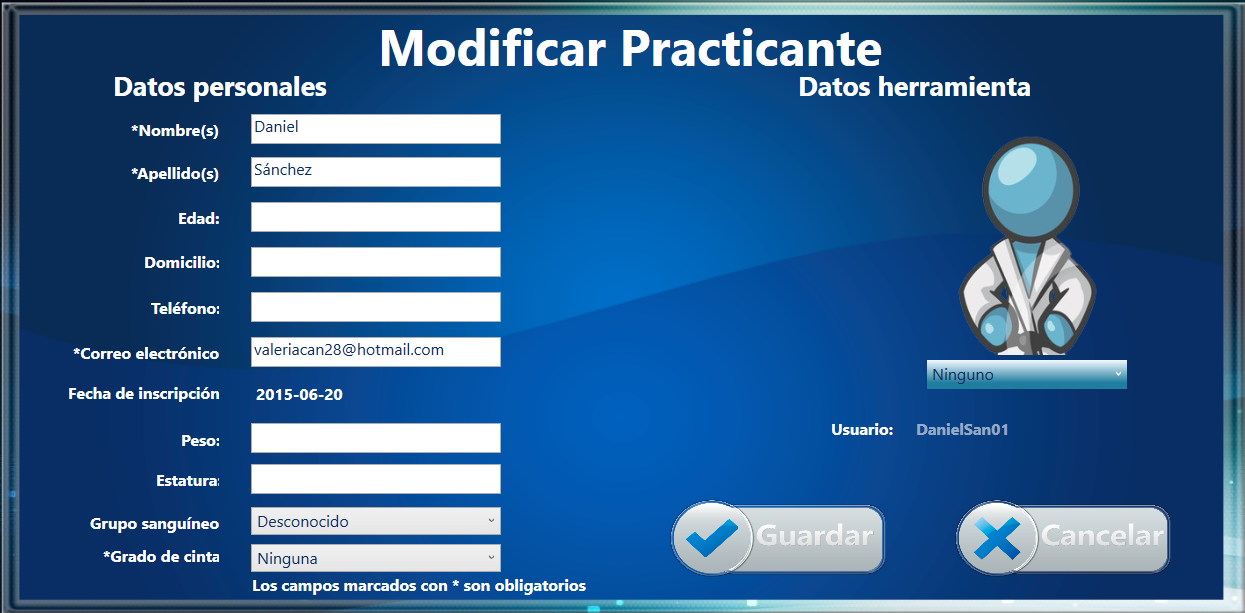
\includegraphics[scale=0.5]{./Figuras/Pantallas/IUE04_1Modificar_informacion_de_Practicante}
	\caption{IUE04.1 Modificar información de Practicante}
	\label{fig:IUE04.1}
\end{figure}

\textbf{\textcolor[rgb]{0, 0, 0.545098}{Entradas}}\\
En esta pantalla el Entrenador deberá capturar la siguiente información:

\begin{itemize}
	\item El/Los Nombre(s).
	\item El/Los Apellido(s).
	\item La Edad.
	\item El Domicilio.
	\item El Teléfono.
	\item El Correo electrónico.
	\item El Peso del Practicante.
	\item La Estatura del Practicante.
\end{itemize}
\vspace{1em}

\textbf{\textcolor[rgb]{0, 0, 0.545098}{Controles}}
\begin{itemize}
	\item \textbf{\textcolor[rgb]{0, 0, 0.545098}{Grupo sanguíneo:}} Permite seleccionar al Entrenador el grupo sanguíneo del Practicante que desea modificar.
	\item \textbf{\textcolor[rgb]{0, 0, 0.545098}{Grado de cinta:}} Permite seleccionar al Entrenador el grado de cinta del Practicante que desea modificar.
	\item \textbf{\textcolor[rgb]{0, 0, 0.545098}{Avatar del Practicante:}} Permite seleccionar al Entrenador un avatar del Practicante que desea modificar.
\end{itemize}
\vspace{1em}

\textbf{\textcolor[rgb]{0, 0, 0.545098}{Comandos}}
\begin{itemize}
	\item \textbf{\textcolor[rgb]{0, 0, 0.545098}{Guardar:}} Permite al Entrenador registrar los nuevos datos del Practicante.
	\item \textbf{\textcolor[rgb]{0, 0, 0.545098}{Cancelar:}} Descarta la nueva información ingresada y regresa a la pantalla \nameref{fig:IUE04}. 
\end{itemize}

\vspace{1em}

\textbf{\textcolor[rgb]{0, 0, 0.545098}{Mensajes}}\\
	
\textbf{\nameref{msj:MSG01}}: Se muestra en la pantalla \nameref{pant:IUE04.1} cuando se modifiquen los datos del Practicante de manera exitosa.\\

\textbf{\nameref{msj:MSG12}}: Se muestra en la pantalla \nameref{pant:IUE04.1} cuando el Entrenador no haya ingresado datos a los campos obligatorios.\\
 
\textbf{\nameref{msj:MSG13}}: Se muestra en pantalla cuando el Entrenador haya ingresado datos con un formato incorrecto en algún campo.\\

\clearpage